\documentclass[12pt,a4paper]{article}
\usepackage[]{listings}
%packages used
\usepackage[english]{babel}
\usepackage[margin=1in,  left=1.25in]{geometry} %margins
\usepackage{pslatex}%Times new roman font
\usepackage{graphicx}%for images
\usepackage{float}
%\usepackage{fancyhdr}
%\pagestyle{fancy}
%\fancyfoot{}

%beginning of document
\begin{document}
%declaration page
%\thispagestyle{empty}
\pagenumbering{roman} 
\begin{titlepage}
  \begin{center}
    \vspace*{1cm}

    \textbf{\Huge Cache report}

    \vspace{0.5cm}

         
    \vspace{1.5cm}

    \textbf{\large Chang Zihao \\20206018\\\large Cui Yuxuan\\20206019}

    \vfill
         

         
    \vspace{0.8cm}
  


         
\end{center}
\end{titlepage}


\newpage
%table of contents
\tableofcontents
\thispagestyle{empty}

\newpage
\pagenumbering{arabic}
\setcounter{page}{1}

\section{Introduction}

Lab5 is required to design a Cache.
A cache processes three state--read and hit, read but miss, and write.
And use cache to save data that use much to save time.
We use multi cycle CPU link the cache.

\subsection{Read Data}

\begin{enumerate}
\item Processor send the address to the cache
\item Then use the valid digit and sign digit to find the data.
\item If the data exist then hit, and send the data to the processor.
\item If the data does not exist then send miss to the memory, the memory will send the data that according to the requirement to the specific position.

\end{enumerate}

\subsection{Write data}

\begin{enumerate}
\item Memory send the address and the data to the cache
\item Then compare the valid digit and sign digit to find the specific position in the cache.
\item Write in the data.

\end{enumerate}

\newpage

\section{Design}

As the Description of TB file mentioned, We do not need to implement memory and register ourselves.
So we design the path to connect them together.

\subsection{Module design}

The PC is a state element that holds the address of the current instruction. 
It is updated at the end of every clock cycle.

\subsubsection{add module}

The adder is responsible for incrementing the PC to hold the address of the next instruction.
It takes two input values, adds them together, and outputs the result

\subsubsection{Sign extend module}

Single extend module is used to increase the number of bits of a binary number while preserving the number's sign and value. 

\subsubsection{MUX module}

Mux, a data selector, which was used to select which the single will be output.


\newpage

\section{Implementation}

\begin{enumerate}
  \item Write-through
  \item Write-allocate
  \item Blocking cache
  \end{enumerate}

Using the write-through policy, data is written to the cache and the backing store location at the same time. 
The significance here is not the order in which it happens or whether it happens in parallel. 
The significance is that I/O completion is only confirmed once the data has been written to both 
places.
Ensures fast retrieval while making sure the data is in the backing store and is not lost in case the cache is disrupted.

Using the Write-allocate, when data is hitten in the cache, just throw the data out.
But if it is missed, the cache needs to ask the memory for the data.

%The whole circuit was shown below.

%\begin{figure}[H]
 % \centering
 % 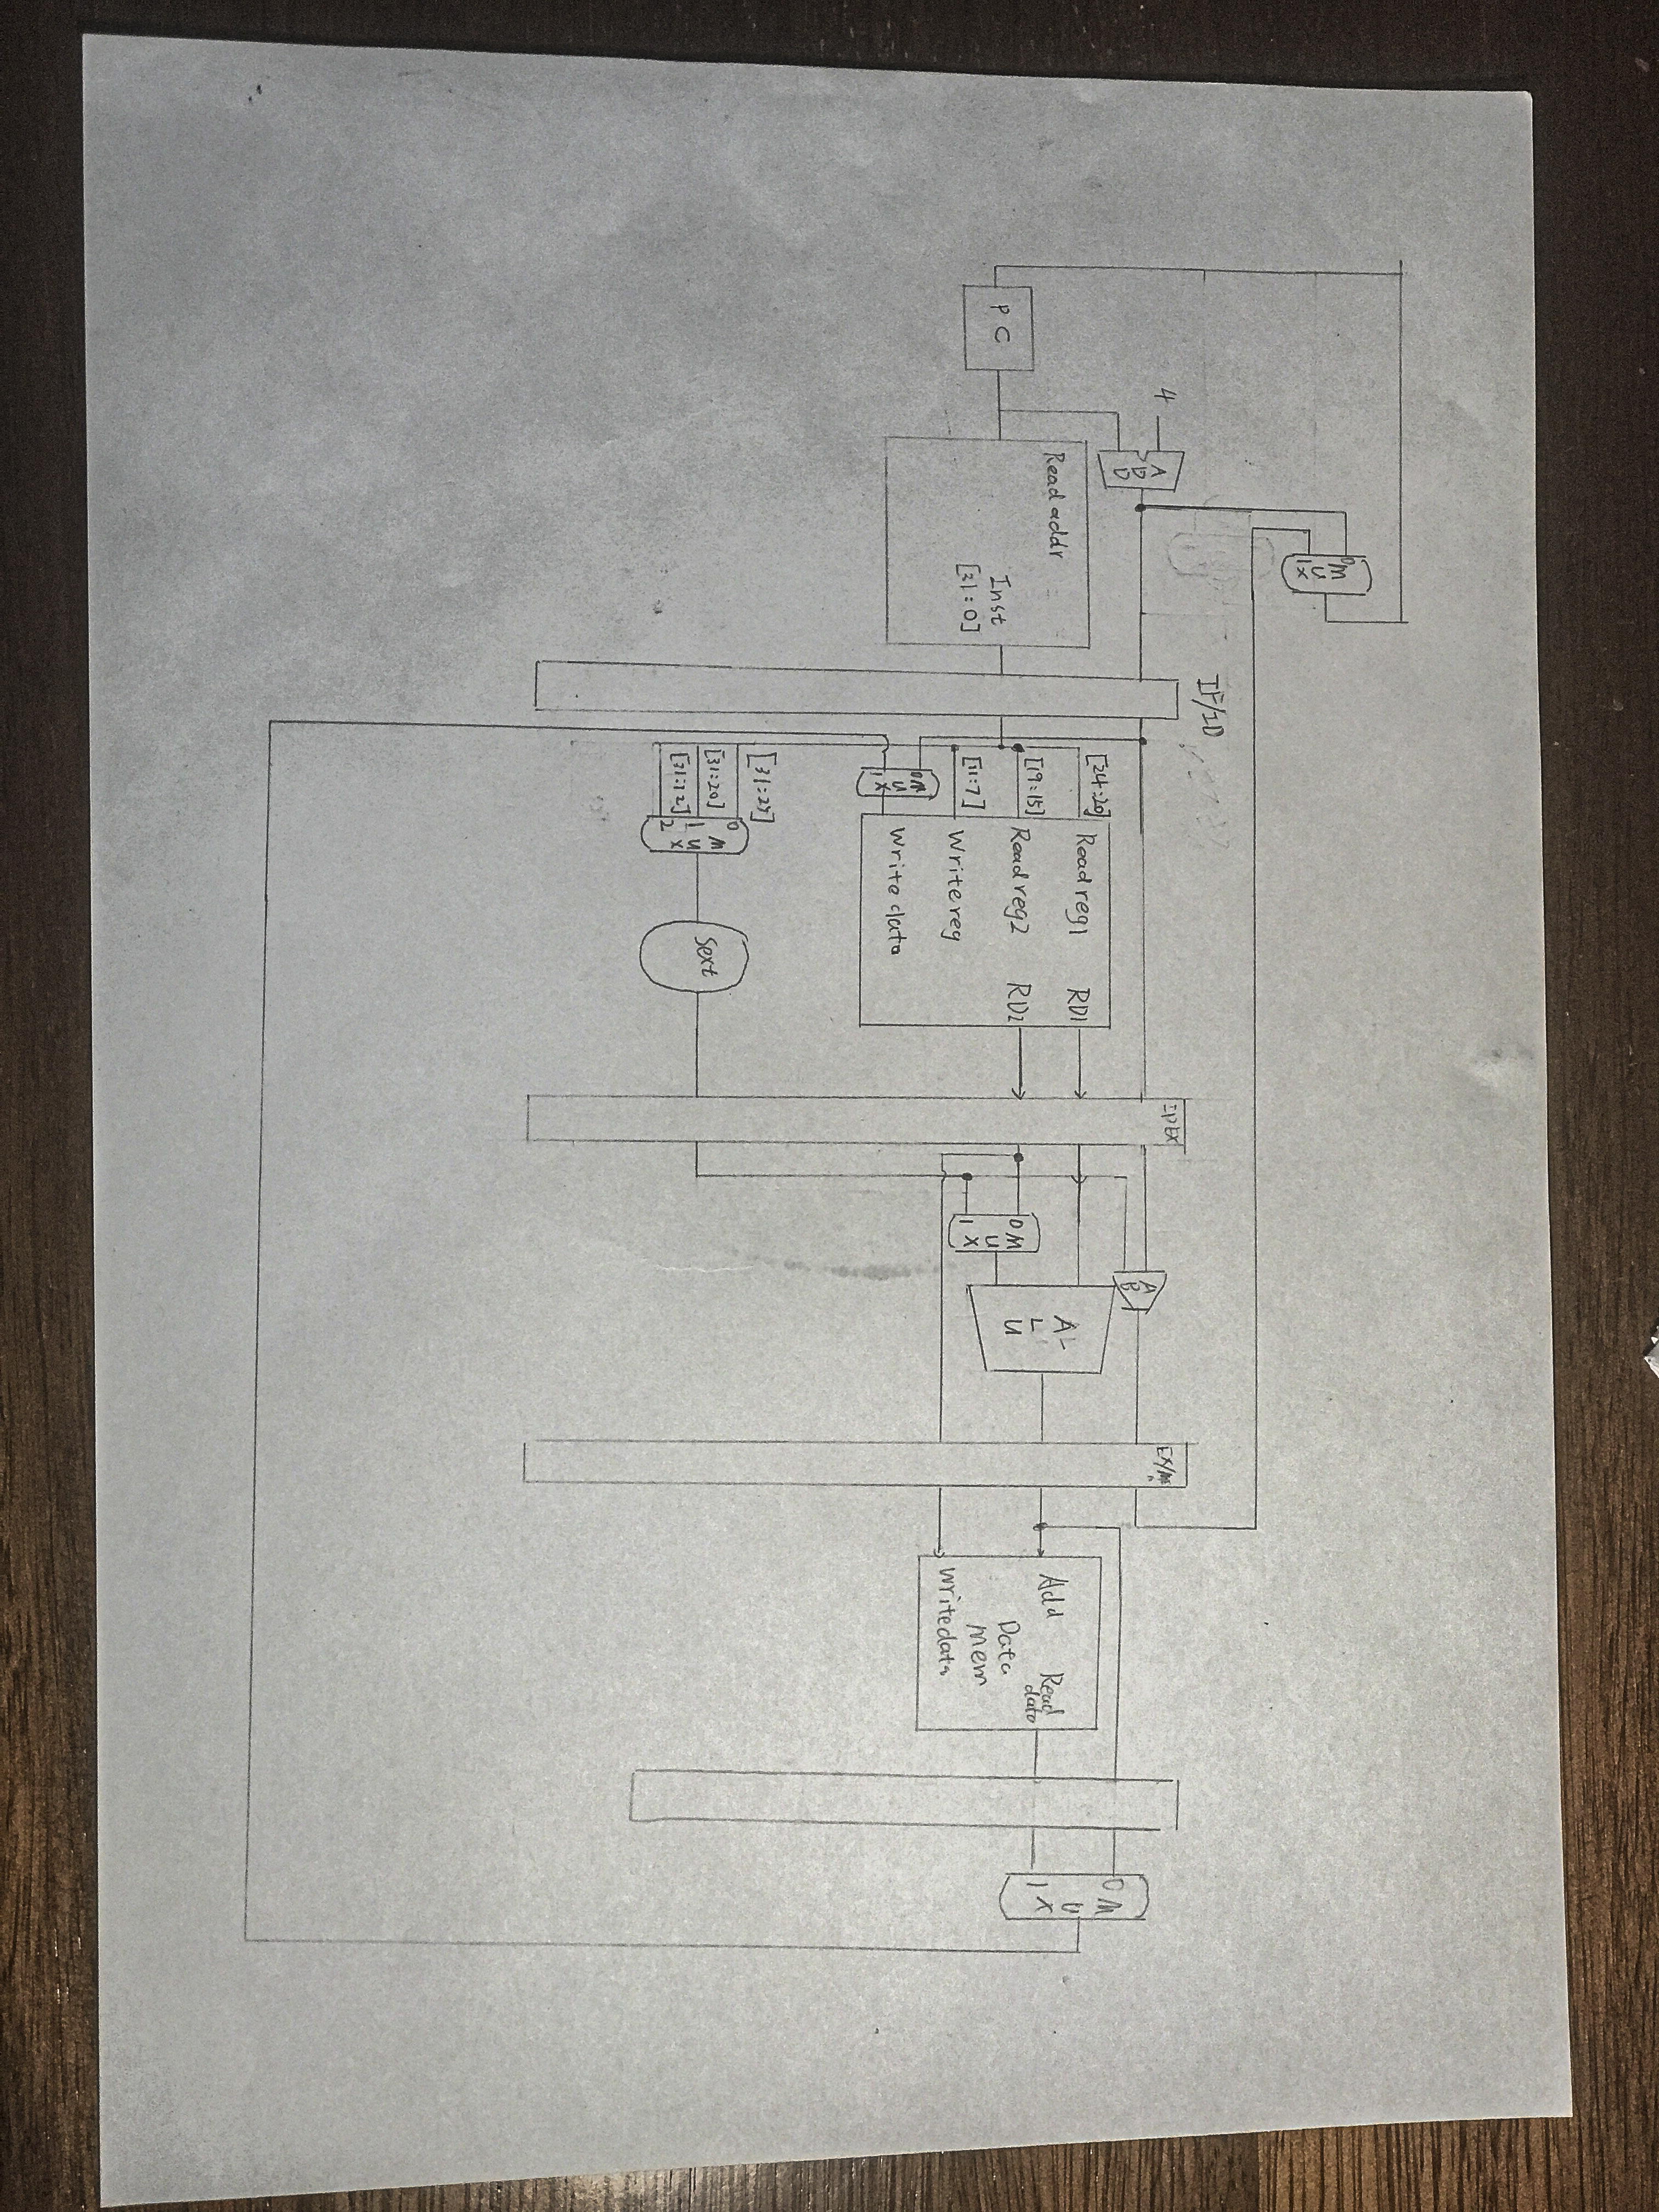
\includegraphics[height=5in, angle=90]{datapath.JPG}
 % \end{figure}
%There might be something different with the circuit.
%  \begin{figure}[H]
%    \centering
%    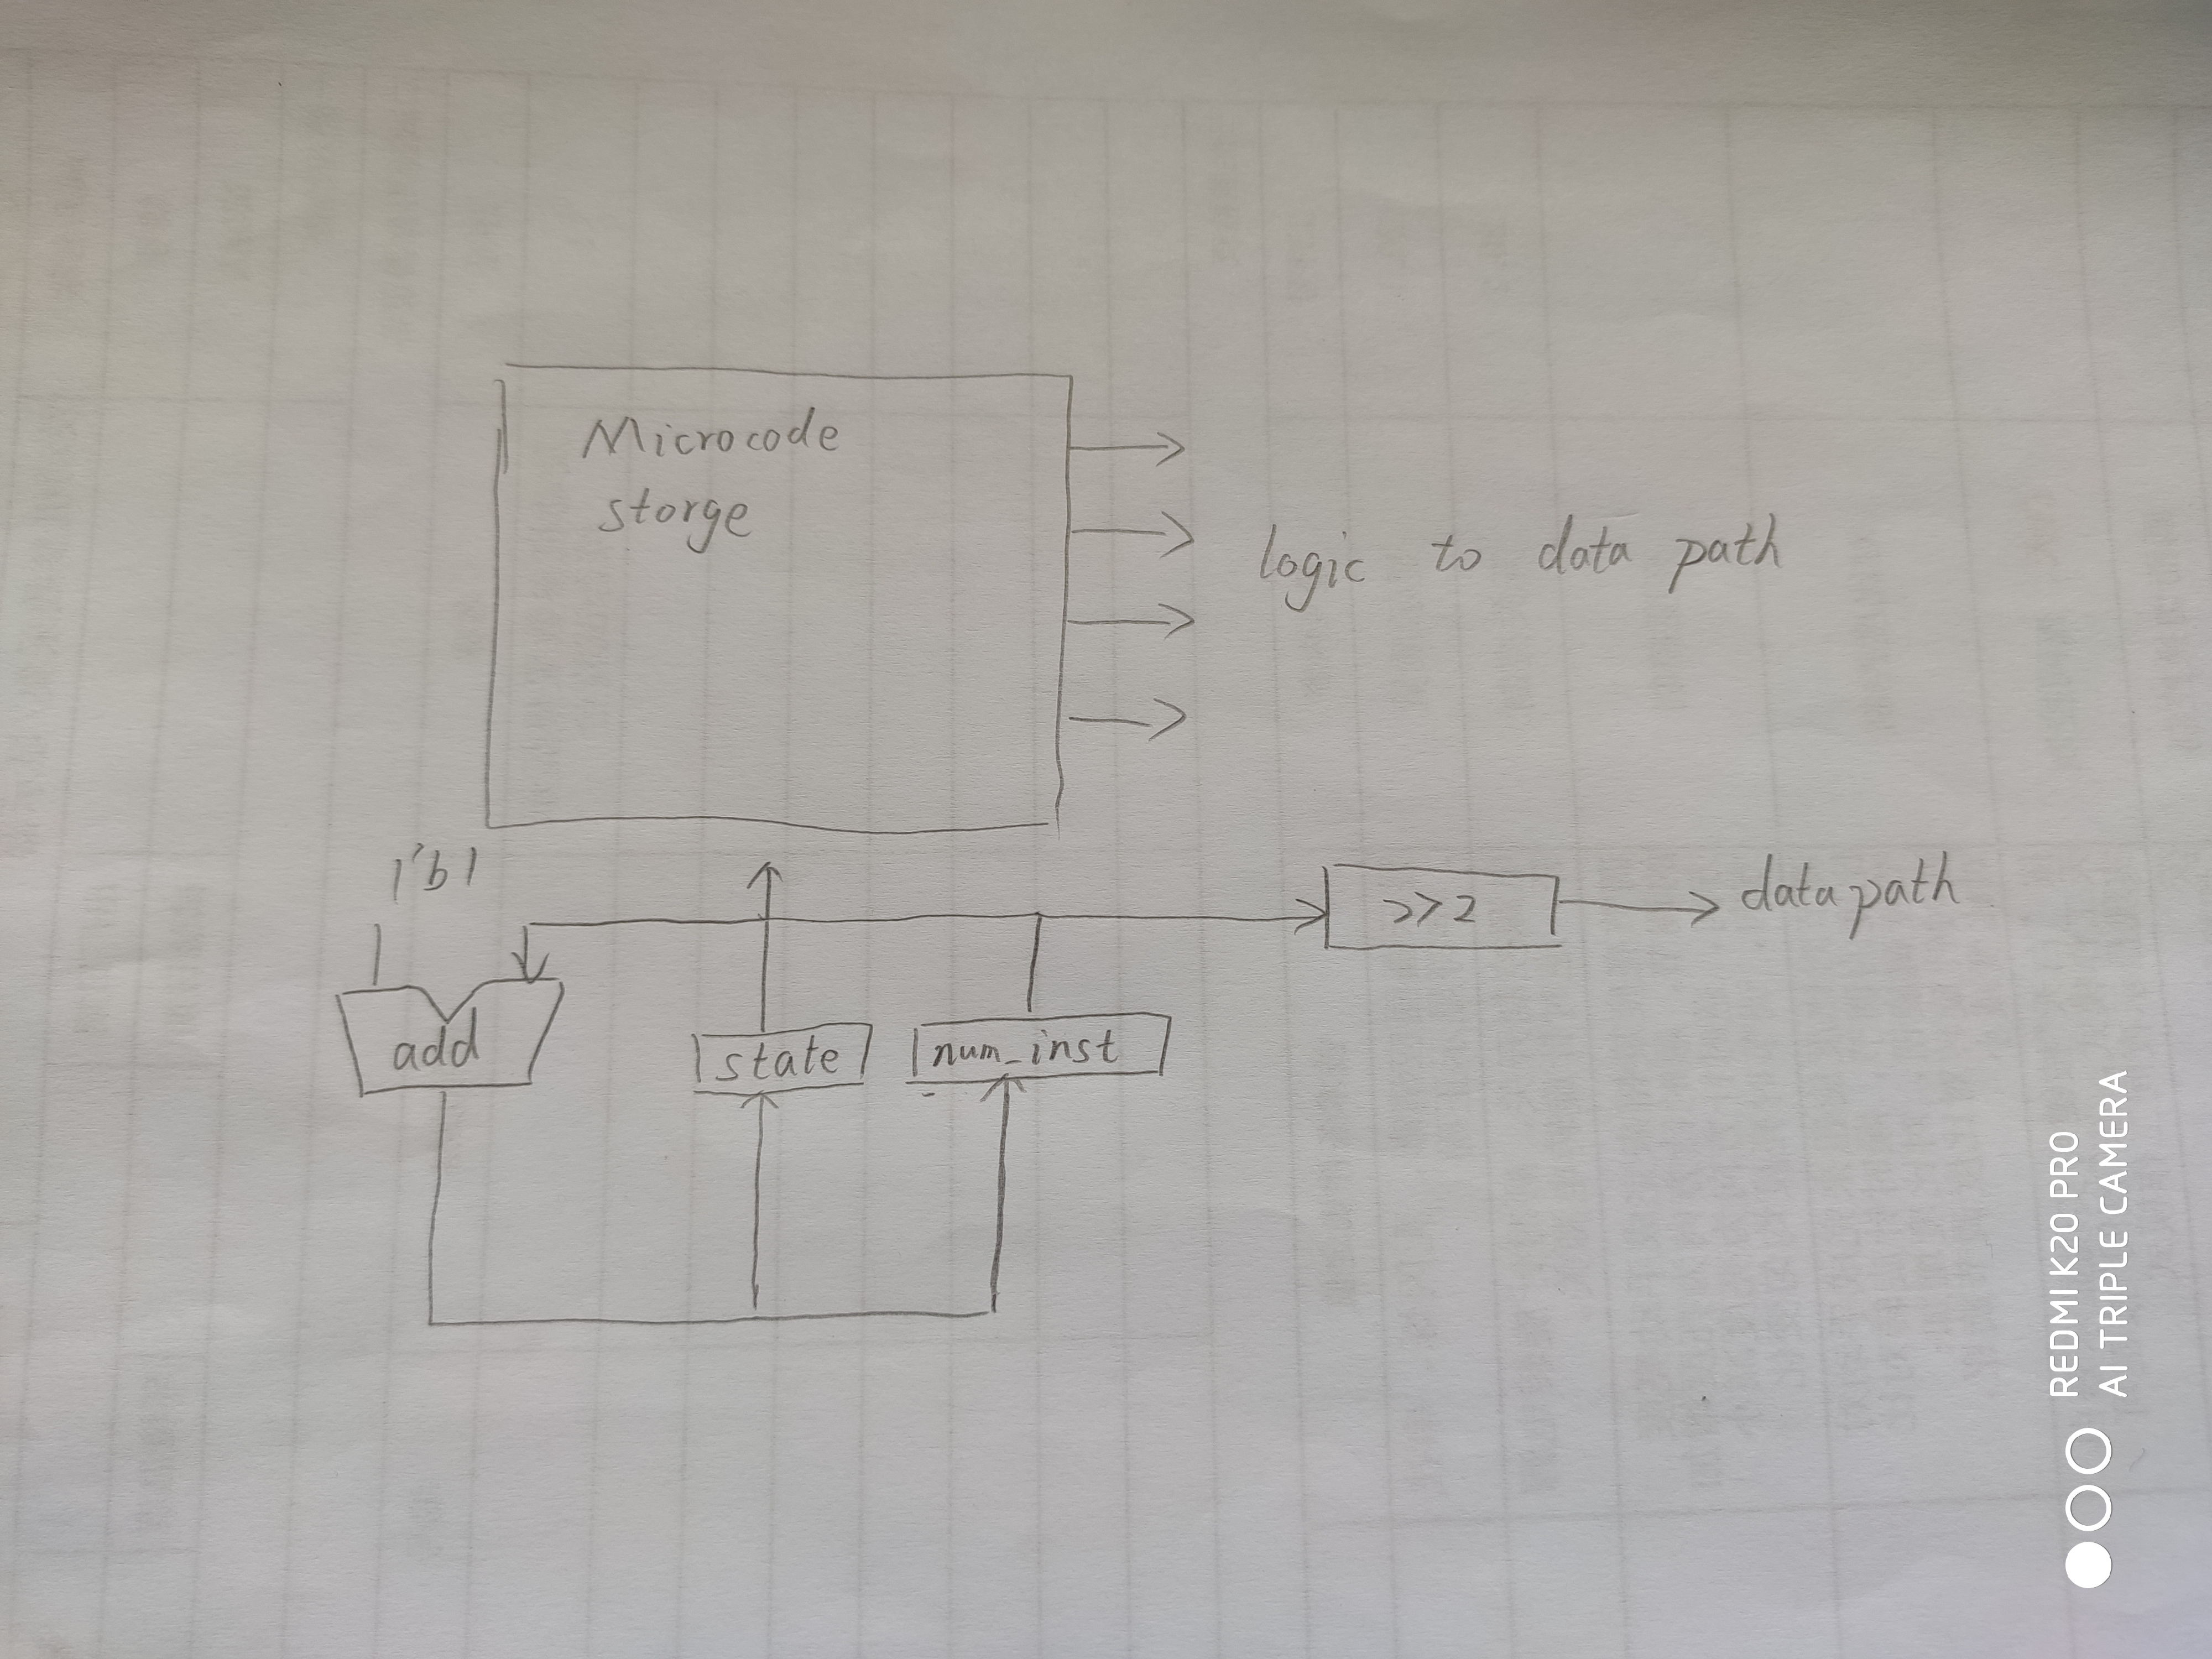
\includegraphics[height=3.5in]{cont.jpg}
%    \end{figure}
\newpage

\section{Evaluation}

I pass all the test in the testbench folder.

\begin{figure}[H]
  \centering
  \includegraphics[height=3in]{inst.PNG}
  \end{figure}

\begin{figure}[H]
  \centering
  \includegraphics[height=3in]{forloop.PNG}
  \end{figure}

  \begin{figure}[H]
    \centering
    \includegraphics[height=2in]{sort.PNG}
    \end{figure}

% We first encountered some problems in understanding the meaning of the question, 
% but in the end by looking at the test code, 
% we thoroughly understood the meaning of the question.
% And at last, we pass all the test and finished the whole project.
% I hope that future projects will give enough time to think and complete the code.

\section{Conclusion}

The cache is very useful in the CPU nowadays,it make the CPU quicker than the CPU last few years.
\end{document}
